\chapter{Aufgaben}\label{chap:Aufgaben}
\section{Aufgaben}\label{sec:sec1}
	\subsection{Aufgabe 1}\label{sub:A1}
	
	Abbildung \ref{plt:Prozess_P} zeigt den Prozess ohne Regler. Der Prozess, in dem Fall der Elektromotor gemeinsam mit dem gesamten mechanischen Aufbau, nimmt als Eingangsgrösse eine Spannung $u(t)$ und setzt als messbaren Ausgang den Winkel $\Theta$ des Pendels. 
	
	%% ---- Plot Prozess alleine
	
\begin{figure}[h]
	\centering
	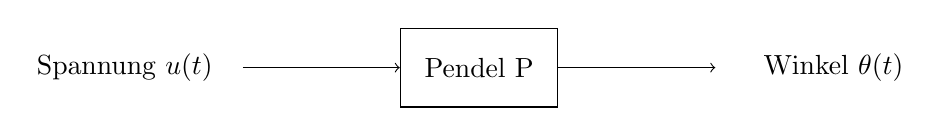
\begin{tikzpicture}
	
	% P-Block
	\node (box) [draw, rectangle, minimum width=2cm, minimum height=1cm] at (3,0) {Pendel P};
	
	% Eingangs-Pfeil 
	\node (input) [left] at (0,0) {};
	\node at (-1.5,0) {Spannung $u(t)$};
	\draw[->] (input) -- (box);
	
	% Ausgangs-Pfeil
	\node (output) [right] at (6,0) {};
	\node at (7.5,0) {Winkel $\theta(t)$};
	\draw[->] (box) -- (output);
	
		\end{tikzpicture}
\caption{Blockschaltbild Prozess}
\label{plt:Prozess_P}
\end{figure}


In Abbildung \ref{plt:Regelkreis_theta} ist der Regelkreis für den Armwinkel $\theta$ dargestellt. Dabei wird aus dem Regelfehler eine Spannung $u(t)$ erzeugt, mit welcher das Pendel entsprechend angesteuert wird. 



%% ---- Plot Regelkreis nur Theta

\begin{figure}[h]
	\centering
	\begin{tikzpicture}[node distance=2cm]
		
      % Eingangsgröße
	\node (r) {};
	
	% Summenpunkt
	\node[circle, draw, right=of r] (sum) {};
	\node[below right=0.2pt and 0.1pt of sum] {$-$};
	\node[above left =2pt and 2pt of sum] {$+$};
	
	% Regler
	\node[draw, rectangle, minimum width=1cm, minimum height=1cm,,right=of sum] (controller) {C $\frac{\theta}{u}$};
	
	% Strecke
	\node[draw, rectangle,  minimum width=1cm, minimum height=1cm, right=of controller] (plant) {P};
	
	% Ausgang
	\node[right=of plant] (y) {};
	
	% Verbindungslinien
	\draw[->] (r) -- (sum) node[midway, above]  {$\theta_{ref} (t) $};
	\draw[->] (sum) -- (controller) node[midway, above] {$\theta_{\text{err}}$};
	\draw[->] (controller) -- (plant) node[midway, above] {$u(t)$};
	\draw[->] (plant) -- (y)  node[midway, above]  {$\theta (t)$};
	
	% Rückführung: von Linie abzweigen und unten herum zurück
	\coordinate (tap) at ($(plant)!0.5!(y)$); % Punkt auf der Linie zwischen plant und y
	\coordinate (feedback) at ($(sum)+(0,-2)$); % Punkt unterhalb des Summenpunkts
	
	\draw[->] (tap) |- (feedback) -| (sum);
		
	\end{tikzpicture}
	\caption{Regelkreis theta}
	\label{plt:Regelkreis_theta}
\end{figure}


%% ---- Plot ganzer Regelkreis

In Abbildung~\ref{plt:Regelkreis_gesamt} ist der gesamte Regelkreis gezeigt. Der äussere Regelkreis gibt dem inneren die Grösse $\theta$ vor, welcher dann wiederrum dieses $\theta$ einzuregeln versucht, ohne dass das Pendel herabstürzt. Mit dieser Kaskadenregelung wird sowohl der Motorenwinkel $\varphi$ als auch der Pendelwinkel $\theta$ geregelt. 

Mit P2 wird der Motor modelliert und mit P1 das Armgelenk. 

\begin{figure}[h]
	\centering
	\begin{tikzpicture}[node distance=1.5cm]
		
		% Eingangsgrösse
		\node (phi_in) {};
		
		% Summenpunkt vor C1
		\node[circle, draw, right=of phi_in] (sum_c1) {};
		\node[below right=0.2pt and 0.1pt of sum_c1] {$-$};
		\node[above left =2pt and 2pt of sum_c1] {$+$};
		
		% Regler C1
		\node[draw, rectangle, minimum width=1cm, minimum height=1cm,,right=of sum_c1] (C1) {C1$\frac{\theta}{\phi}$};

		% Summenpunkt vor C2
		\node[circle, draw, right=of C1] (sum_c2) {};
		\node[below right=0.2pt and 0.1pt of sum_c2] {$-$};
		\node[above left =2pt and 2pt of sum_c2] {$+$};
		
		% Regler C2
		\node[draw, rectangle, minimum width=1cm, minimum height=1cm,,right=of sum_c2] (C2) {C2$\frac{u}{\theta}$};
		% Strecke  P2
		\node[draw, rectangle,  minimum width=1cm, minimum height=1cm, right=of C2] (P2) {P2};
		
		% Strecke  P1
		\node[draw, rectangle,  minimum width=1cm, minimum height=1cm, right=of P2] (P1) {P1};
		
		% Ausgang Phi
		\node[right=of P1] (phi_out) {};
		
		% Verbindungslinien
		\draw[->](phi_in) -- (sum_c1) node[midway, above]  {$\varphi_{ref} (t)$};
		\draw[->](sum_c1) -- (C1) node[midway, above] {$\varphi_{err} (t)$};
		\draw[->](C1) -- (sum_c2) {} node[midway, above]  {$\theta_{ref}$};
		\draw[->](sum_c2) -- (C2) node[midway, above] {$\theta_{err}$};
		\draw[->](C2)--(P2) node[midway, above] {$u(t)$};
		\draw[->](P2)--(P1) node[midway, above] {$\theta (t)$};
		\draw[->](P1) -- (phi_out) node[midway, above]  {$\varphi (t)$};
		
		% Rückführung: innerer Kreis
		\coordinate (p_output_inner_circle) at ($(P2)!0.5!(P1)$); 
		\coordinate (p_target_sum_inner_circle) at ($(sum_c2)+(0,-1)$); 
		\draw[->] (p_output_inner_circle) |- (p_target_sum_inner_circle) -| (sum_c2);
		
		% Rückführung: äusserer Kreis
		\coordinate (p_output_outer_circle) at ($(P1)!0.5!(phi_out)$); 
		\coordinate (p_target_sum_outer_circle) at ($(sum_c1)+(0,-2)$); 
		\draw[->] (p_output_outer_circle) |- (p_target_sum_outer_circle) -| (sum_c1);
				
		
	\end{tikzpicture}
	\caption{Regelkreis Pendel}
	\label{plt:Regelkreis_gesamt}
\end{figure}


\subsection{Aufgabe 2}\label{sub:A2}

Der Prozess ist weder Stabil, noch linear. Daher ist bereits von Seiten der Vorbereitung auf diesen Versuch die linearisierte Übertragungsfunktion hergeleitet worden. 

\begin{align}
	\ddot{\varphi}(t) &= 	\frac{-\mu A_v - \frac{K_m^2 G}{R}}{J_A + m_2 L_1^2} \, \dot{\varphi}(t) 	+ \frac{m_2 L_1 l_2}{J_A + m_2 L_1^2} \, \ddot{\theta}(t) + \frac{G K_m}{R \left(J_A + m_2 L_1^2\right)} u(t) \\[10pt]
	\ddot{\theta}(t) &= \frac{m_2 L_1 l_2}{J_P} \, \ddot{\varphi}(t) - \frac{\mu P_v}{J_P} \, \dot{\theta}(t) + \frac{m_2 g l_2}{J_P} \, \theta(t)
	\end{align}

Um die Berechnungen im folgenden zu vereinfachen, werden die linearisierten Übertragungsfunktionen wie folgt vereinfach: 

\begin{align}
	\ddot{\varphi}(t) &= 	A \, \dot{\varphi}(t) 	+ B \, \ddot{\theta}(t) +C \, u(t) \\[10pt]
	\ddot{\theta}(t) &= \alpha \, {\varphi}(t) -\beta \, \dot{\theta}(t) + \gamma \, \theta(t)
	\end{align}

Damit ergeben sich die Übertragungsfunktionen wie folgt: 

\begin{align}
	\frac{\Theta(s)}{U(s)} & = \frac{C \alpha s} {s^3 - s^2 (\beta + A) - s (\gamma - A \beta) + A \gamma }                                      \\[10pt]
	\frac{\Phi (s)}{U (s)} & =  \frac{C (s^2 - \beta s - \gamma) } {s^4 (1 - \alpha B) - s^3 (\beta + A ) - s^2 (\gamma - A \beta) + s A \gamma}
\end{align}


\subsection{Aufgabe 3}

Die Parameter sind entweder aus Datenblättern entnommen, oder aus Berechnungen hergeleitet.
Die für das in den Aufgaben verwendete Modell verwendeten Parameter sind Tabelle\ref{tab:parameter_modell} zu entnehmen. 

\begin{table}[h]
	\centering
	\begin{tabular}{l|l}
		\textbf{Parameter} & \textbf{Wert}                        \\ \hline
		$L_1$               & $0.147425 \, \text{m}$               \\
		$l_2 $              & $0.116569 \, \text{m}$               \\
		$m_2$               & $0.018 \, \text{kg}$                 \\
		$R $               & $0.74 \, \Omega$                     \\
		$k_{m}$            & $21.4 \times 10^{-3} \, \text{Nm/A}$ \\
		$G$                & $\frac{5625}{361}$
	\end{tabular}
	\caption{Parameteridentifikation}
	\label{tab:parameter_modell}
\end{table}


\subsection{Aufgabe 4}










